\chapter{Revisão bibliográfica}
\label{cap:fundamentacao-teorica}
Este capítulo investiga o panorama atual das pesquisas sobre o tema, explorando as contribuições relevantes e as lacunas existentes no desenvolvimento de projetos anteriores.

\section{Problematização}

A ocupação do ser humano no contexto social rege-se de diversas atividades rotineiras que agregam propósito e significado à vida. Elas são divididas em três grupos principais, sendo: Atividades de Vida Diária (AVD), Atividades Instrumentais de Vida Diária (AIVD), Sono e descanso, Trabalho, Brincar, Lazer, Participação social e Educação \cite{aota}. Desde a manutenção de necessidades vitais à realização pessoal em contextos familiares, educacionais e profissionais, esses compromissos podem variar em priorização e grau de importância a cada indivíduo. Contudo, fatores socioeconômicos, ambientais e relações interpessoais desempenham um papel influente quanto à realização dessas atividades para a continuidade de uma vida equilibrada e saudável.

Historicamente, é possível observar que o grau de disponibilidade de ferramentas para realização de tarefas ocupacionais é resultado de uma desigualdade de oportunidades entre diferentes grupos sociais. Neste sentido, ao focalizar a lente em pessoas com deficiência, a disparidade social relativa à inclusão em atividades diárias mostra-se ainda mais latente.

Nesse contexto, o uso de Tecnologia Assistiva assume uma relevância ainda maior, tornando-se uma abordagem crucial para minorar as barreiras funcionais específicas da deficiência visual. O termo refere-se a um arsenal de equipamentos, recursos e estratégias voltados à potencialização das habilidades práticas de pessoas com deficiência \cite{TecnologiaAssistivaDeficienciaVisual}, facilitando ou possibilitando a atuação em diversas atividades ocupacionais. Os elementos da Tecnologia Assistiva visam facilitar a execução das atividades cotidianas de maneira mais independente, reduzindo a dependência e promovendo uma participação mais ativa. Isso permite um desempenho aprimorado, especialmente para aqueles que enfrentam desafios relacionados à deficiência física e/ou visual \cite{BarreirasArquitetonicas}.

No contexto de sistemas computacionais, a implementação de tecnologias assistivas requer acessibilidade a fim de permitir a usabilidade, garantindo o propósito do sistema. Em outras palavras, para que as funcionalidades possam ser aproveitadas em sua totalidade por usuários, é necessário que o usuário possa interagir com a interface sem obstáculos ou barreiras \cite{BarbosaSilva2010}. 

Entretanto, mesmo com o desenvolvimento de ferramentas que buscam melhorar a experiência de pessoas com deficiência no que tange à interação com o espaço físico e social, ainda existem lacunas para a devolução de autonomia a esses indivíduos. Uma dificuldade apresentada na expansão de tecnologias assistivas voltadas à inclusão dessas pessoas reside-se no fato de que a maioria dos desenvolvedores, projetistas e designers não possuem problemas na visão. Assim, quando as necessidades específicas dessa parcela de usuários não são levadas em consideração ao longo do processo de desenvolvimento e testes, é possível que o projeto afaste-os como potenciais utilizadores do sistema. Portanto, a não-inclusão desse grupo acaba retroalimentando a sua exclusão em atividades diárias. 

Por outro lado, a abordagem de tecnologias assistivas voltadas a pessoas com deficiência visual pode ficar bastante concentrada na questão da usabilidade de aplicações e interfaces acessíveis, entretanto, nota-se a ausência de projetos voltados à inclusão desse grupo também no ambiente espacial. Uma revisão de escopo realizada por Zen et al. (2022) possui o propósito de analisar pesquisas recentes em termos de Tecnologia Assistiva voltada à interação de usuários para obter uma visão ampla da área. Após a análise e filtragem consecutiva de artigos produzidos sobre o uso de Tecnologias Assistivas no contexto de Inteligência da Informação, constatou-se que menos de 5\% dos trabalhos produzidos possuíam enfoque de auxiliar Orientação e Mobilidade com o uso de TAs  \cite{TecnologiaAssistivaDeficienciaVisual}.

Outrossim, a experiência interativa para com o ambiente ao redor é bastante diferente entre pessoas com alguma dificuldade visual e indivíduos sem nenhum obstáculo para enxergar. Apesar da Lei da Acessibilidade, Nº 10.098, publicada no ano 2000, preconizar normas e critérios básicos para garantir a acessibilidade de pessoas com deficiência também em espaços urbanos, ela só pode ser cobrada em construções posteriores ao seu estabelecimento. Dessa forma, embora proponha sinalização sonora, guia, cores e iluminações, uma boa área do espaço arquitetônico não está abrangendo as normas estabelecidas.

A Lei 10.098 foi reforçada com parâmetros de acessibilidade que devem ser aplicados em edificações através do manual da ABNT 9050 em 2004. Todavia, um estudo realizado por Neves et al. (2021) mostra a análise de diversos elementos em uma instituição educacional situada em Belém - PA. Os resultados delineiam obstáculos que pessoas com deficiência, sobretudo visual e motora, encontram nesses espaços. Dentre as características observadas, notam-se a ausência de mapa tátil, ruas desniveladas, calçadas altas, pinturas apagadas e cores sem contraste \cite{BarreirasArquitetonicas}.  

Dado o exposto, fica evidente que o ambiente urbano não é totalmente adequado para que pessoas com deficiência visual possam se locomover com segurança e independência. Essa hostilidade do espaço arquitetônico, somada à ausência de pesquisas voltadas ao uso de tecnologias assistivas no auxílio desse grupo, fortalecem a oportunidade de desenvolver ferramentas para devolver autonomia a esses indivíduos pouco favorecidos por políticas de acessibilidade e inserção no meio social. É nesse contexto em que se torna importante o desenvolvimento de novos recursos, com o auxílio da tecnologia, visando fomentar a inclusão e assegurar que os indivíduos com limitações visuais tenham paridade de acesso e oportunidades no contexto urbano.

\section{Análise literária}
Em função de entender melhor as questões pontuais enfrentadas por pessoas com deficiência visual, foi realizada uma análise literária de projetos que contam com pesquisa de campo com o propósito de entender a relação entre esses indivíduos e os obstáculos identificados em sua mobilidade. Dessa forma, foram analisados três trabalhos para o levantamento dos dados, feitos por Clara de Castro Marinho (2020), Alessandro Cardozo Bueno (2010) e Costa \textit{et al.} (2020).

\subsection{ Dispositivos Vestíveis para o Auxílio na Locomoção de Pessoas com Deficiência Visual
}

As entrevistas realizadas neste trabalho foram realizadas com doze pessoas com cegueira entre 18 a 51 anos, de acordo com a classificação sugerida pela OMS, identificada no Quadro 1. Os questionamentos foram realizados de maneira remota, seja por ligações telefônicas ou chamadas de vídeo, e possuíam o objetivo de compreender melhor o público-alvo e analisar as experiências vividas por pessoas com deficiência visual, identificando as dificuldades enfrentadas por elas ao se deslocar pelo ambiente urbano a pé.

Os entrevistados forneceram informações sobre o grau de deficiência, o uso de recursos de locomoção, a frequência e os destinos dos seus deslocamentos, e as dificuldades encontradas ao caminhar nas vias urbanas. A maioria dos entrevistados relatou o uso da bengala como principal recurso assistivo, além de aplicativos como GPS e Google Maps. Os obstáculos mais comuns mencionados foram calçadas irregulares, postes, árvores, e a ausência de piso tátil.

Sobre os acessórios de uso diário, foram citados pulseiras, óculos, brincos e colares. Quanto ao produto a ser desenvolvido, as sugestões incluíram: um dispositivo pequeno, leve, fácil de manusear e acoplar ao corpo; integração com aplicativos de celular via Bluetooth; e preferência por emissão de sons ao invés de vibrações. Todos os entrevistados demonstraram grande interesse no uso do produto e acreditam que a adaptação não seria um problema. A maioria afirmou que utilizaria o produto em conjunto com outros recursos assistivos, como a bengala \cite{claramarinho-2020}.

\subsection{Bengala Eletrônica para Deficientes Visuais}

A pesquisa realizada por Bueno (2010) foi desenvolvida no Instituto Paranaense de Cegos (IPC), localizado em Curitiba. Nessa pesquisa, foi questionada ao público-alvo a real necessidade de pessoas com deficiência visual em utilizar uma bengala eletrônica, o preço que estariam dispostas a pagar, os desconfortos encontrados nas atuais bengalas e quais os recursos mais eficazes atualmente para promover a locomoção de maneira segura.

Como resultado da pesquisa, o autor levantou que as bengalas tradicionais não são completamente eficientes por não identificarem obstáculos suspensos em relação ao solo, causando acidentes recorrentes. Além disso, a maior parte das pessoas entrevistadas não realizava uma atividade remunerada e, nos casos em que havia uma fonte de renda, esta não era satisfatória. Dessa forma, foi determinado que a bengala automatizada deveria ter um baixo custo para requisição e manutenção.

Por fim, os entrevistados mencionaram que o melhor recurso existente para promover uma locomoção segura era o cão-guia. Entretanto, os custos de treinamento e obtenção do cachorro costumam ser bastante elevados, dificultando a utilização deste recurso por parte de pessoas com deficiência visual \cite{bueno-2010}.

\subsection{Desenvolvimento de uma Bengala Automatizada Utilizando Arduino para Deficientes
Visuais}

Esta pesquisa foi realizada com quatro alunos do Centro Municial de Educação Especial Prof. Isoldi Storck, que atende pessoas com deficiência visual e auditiva, com o objetivo principal de coletar dados para nortear a criação de uma tecnologia sensorial para aumentar a acessibilidade de indivíduos com cegueira. A pesquisa, dividida em duas etapas e utilizando questionários, envolveu métodos quantitativos e qualitativos.

Na primeira etapa, antes da criação da bengala automatizada, foram entrevistados quatro alunos para entender suas necessidades e a viabilidade do projeto. As perguntas abordaram questões como acessibilidade, frequência de acidentes e a percepção sobre a utilidade de uma tecnologia sensorial para locomoção. Com base nas respostas, a bengala foi desenvolvida e posteriormente testada na segunda etapa da pesquisa.

Após a montagem da bengala, a equipe retornou à instituição para avaliar o protótipo. Os alunos testaram a bengala e responderam a um segundo questionário, que revelou que a bengala ajudou de maneira eficaz na locomoção segura, com a maioria dos entrevistados manifestando interesse em usar a tecnologia no cotidiano. No entanto, foram sugeridas melhorias, como aumentar o comprimento, reduzir o peso e tornar a bengala dobrável para facilitar o transporte. A pesquisa concluiu que a bengala atingiu seus objetivos iniciais, mas que implementações adicionais poderiam torná-la mais confortável e prática para os usuários.

\subsection{Conclusões}
Os três trabalhos analisados contribuíram para o desenvolvimento de tecnologias assistivas voltadas para a mobilidade de pessoas com deficiência visual. As entrevistas e pesquisas de campo realizadas revelaram a importância de criar dispositivos acessíveis, práticos e adaptáveis às necessidades dos usuários. As sugestões dos entrevistados foram cruciais para direcionar as melhorias nos projetos, como a integração com tecnologias móveis, a redução de peso, e o ajuste de tamanho das bengalas automatizadas. Além disso, ficou evidente que a acessibilidade urbana ainda enfrenta muitos desafios, como a presença de obstáculos e a falta de sinalização adequada, reforçando a necessidade de soluções inovadoras que possam ser utilizadas em conjunto com os recursos assistivos tradicionais. Esses trabalhos reforçam a importância de um design centrado no usuário para desenvolver tecnologias que realmente atendam às demandas específicas das pessoas com deficiência visual, promovendo maior autonomia e segurança em sua locomoção diária.

\section{Projetos Anteriores}
Na história da literatura, podemos encontrar exemplos de projetos semelhantes que surgiram no ambiente acadêmico, abordando propostas similares em relação à expansão de tecnologias assistivas \cite{Rigolon} \cite{BengalaAutomatizadaArduino}. No entanto, é notável a falta de continuidade do desenvolvimento desses recursos ao longo do tempo, o que se reflete na escassez de produtos disponíveis para atender às necessidades do público-alvo. Essa lacuna persistente, seja através do mercado convencional ou de iniciativas assistenciais, evidencia um desafio significativo na área.

Dentre os projetos encontrados em pesquisas e revisões bibliográficas, destaca-se o uso recorrente de tecnologias como sensores ultrassônicos e motores de vibração acoplados a microcontroladores com chip ATmega328. Esses componentes são frequentemente empregados como funcionalidade principal em dispositivos e sistemas desenvolvidos para abordar questões específicas, como acessibilidade, autonomia e segurança.

A frequente utilização desses componentes em projetos com o propósito de identificar objetos deve-se, principalmente, pelo baixo custo das peças, disponibilidade no mercado e eficiência. No artigo produzido por Lima \textit{et al.} (2015), no qual os autores descrevem o processo de desenvolvimento de uma bengala automatizada, foram apresentadas outras opções de componentes avaliadas e a justificativa da escolha para cada categoria. 

    \subsection{Projeto de Equipamento Sensorial para Orientação e Mobilidade de Deficientes Visuais}\label{sec:citacoes}
    
        O projeto de equipamento sensorial \cite{Rigolon}, para o Bacharelado em Engenharia Eletrônica, enfoca-se em um projeto de equipamento sensorial para orientação e mobilidade de deficientes visuais. O objetivo da ferramenta é identificar obstáculos acima da linha da cintura do usuário. Nesse sentido, conta com a utilização de um sensor ultrassônico HC-SR04, um motor de vibração de celular e um microcontrolador acoplados próximo à palma da mão.
    
        O modo de vibração do projeto apresentado por Almeira e Rigolon alterna-se a depender da distância do objeto. A vibração é intermitente e torna-se mais frequente conforme o usuário se aproxima do obstáculo. Assim, o dispositivo transmite níveis diferentes de sensibilidade para o usuário.
    
        Todavia, não houve indicação de como o protótipo foi energizado. Os autores descreveram um caso de teste no qual o dispositivo foi utilizado diante de uma caixa grande de MDF como protótipo. Assim, com linhas medidas no chão, verificou-se que a distância estava sendo mensurada corretamente e, portanto, o motor de vibração emitia os sinais esperados. Contudo, não foi mencionado o uso de nenhuma bateria ou fonte de energia externa para manter o circuito energizado. Portanto, a ausência de informações sobre a fonte de energia utilizada para alimentar o dispositivo sensorial apresentado pelos autores pode indicar uma limitação significativa em relação à viabilidade prática do protótipo. Sem uma fonte de energia definida, a portabilidade e autonomia do dispositivo podem ser comprometidas, dificultando sua utilização no dia a dia por parte dos usuários.
    
    \subsection{Desenvolvimento de uma Bengala Automatizada Utilizando Arduino para Deficientes Visuais}

        Similarmente, o trabalho refere-se a um protótipo de uma bengala automatizada \cite{BengalaAutomatizadaArduino}, com o propósito de identificar objetos na altura do peito e do solo. Assim, conta com dois sensores ultrassônicos na extensão da bengala que detectam objetos entre 30cm até 200cm, de forma que um \textit{buzzer} emite um alarme sonoro mais intenso conforme a distância detectada pelos sensores diminui. 
    
        Apesar do microcontrolador ser alimentado por uma bateria de 9V, não há a possibilidade de recarregar o modelo de forma convencional através de uma fonte de energia externa. Embora exista a possibilidade de ligar e desligar a bengala através de uma chave, ampliando a vida útil da bateria, a necessidade de repor as baterias torna o projeto pouco prático no cotidiano.

    \subsection{Comparação de funcionaliades oferecidas}
    
    Os trabalhos desenvolvidos na área anteriormente exploram a possibilidade de utilização de sensores com o propósito de alertar usuários com deficiência visual, melhorando a interação com o meio ambiente. Dessa forma, o presente projeto busca explorar e desenvolver diferentes funcionalidades integradas num único aparelho com o propósito de aumentar o potencial de uso da bengala inteligente. 

    
    O Quadro \ref{tab:comparativo_funcionalidades} apresenta um comparativo das funcionalidades oferecidas pela Bengala Inteligente em relação a dois outros projetos acadêmicos apresentados anteriormente, produzidos por Almeida e Rigolon (2016) e Costa et al. (2020). A revisão desses trabalhos mostrou que é possível desenvolver a bengala inteligente e promover um auxílio na vida de pessoas que pertencem ao público-alvo deste projeto.

        \begin{quadro}[!ht]    
            \captionsetup{width=1.0\textwidth} % Definindo a largura da legenda
            \caption{Comparativo de funcionalidades trazidas pela Bengala Inteligente}    
            \begin{tabular}{p{0.3\textwidth}p{0.2\textwidth}p{0.2\textwidth}p{0.2\textwidth}} % Definindo larguras para as colunas

                \toprule
                Funcionalidades & Bengala Inteligente & RIGOLON e ALMEIDA (2016) & COSTA \textit{et. al.} (2020)  \\
                \midrule
                Bateria                                                 & X  &    & X  \\
                Vibração                                                & X  &  X &    \\
                Identificação de obstáculos na altura do peito          & X  &  X & X  \\
                Identificação de obstáculos na altura do solo           & X  &    & X  \\
                Sons                                                    & X  &    & X  \\
                Reconhecimento de toque                                 & X  &    &    \\
                Recarregamento                                          & X  &    &    \\
                Desligar a bengala                                      & X  &    & X  \\
                \bottomrule
            \end{tabular}
            \caption*{Fonte: elaborada pelos autores.} % Legenda sem rótulo
            \label{tab:comparativo_funcionalidades}

        \end{quadro}
    Assim, dado o exposto, evidencia-se que a bengala inteligente traz funcionalidades úteis que aumentam a utilização prolongada da bengala e fornece uma experiência completa ao usuário. A integração de diferentes tipos de alertas, reconhecimento do toque do usuário, identificação de objetos em diferentes alturas, recarregamento da bengala para aumentar a vida útil e desligamento do sistema são exemplos de funcionalidades que ampliam significativamente a utilidade e a conveniência deste dispositivo assistivo.

    

%    Referenciando outro site \nocite{secretaria1999}(SÃO PAULO, 1999). Neste caso, foi utilizado o comando \verb=\nocite{}=
 %   que faz com que a referência aparaça e em seguida foi escrito manualmente (SÃO PAULO, 1999). Esse recurso foi utilizado porque se existem particularidades ao citar um estado. E não havia uma macro elaborada para esta citação. Assim, sempre que o estila da citação tiver uma particularidade não contemplada pelo nosso modelo, é possível utilizar este recurso manual.
    
  
%  Texto texto texto texto texto texto texto texto texto texto texto texto texto texto texto texto texto texto texto. Texto texto texto texto texto texto texto texto texto texto texto texto texto texto texto texto texto texto texto. Citando uma norma \cite{NBR10520:2002}.
        
 %   Citação de duas referências que concordam entre si \cite{Almeida2018,Gondim2017}. Texto texto texto texto texto texto texto texto texto texto texto texto texto texto texto texto texto texto texto. Texto texto texto texto texto texto texto texto texto texto texto texto texto texto texto texto texto texto texto. Texto texto texto texto texto texto texto texto texto texto texto texto texto texto texto texto texto texto texto. Texto texto texto texto texto texto texto texto texto texto texto texto texto texto texto texto texto texto texto texto texto texto texto texto texto texto. Citando um manual \nocite{manuais1989}(SÃO PAULO, 1989). 
        
 %  Outro tipo de citação é a citação literal ou direta com mais de três linhas. Este tipo de citação deve ser destacada com recuo de $4~cm$ da margem esquerda com letra menor (tamanho 10), sem aspas e com espaçamento simples.  Para exemplificar esse tipo de citação, considere a afirmação de \citeonline[p.~98]{feitosa2016}:
  %  \begin{citacao}
  %      A cultura é o processo através do qual o homem cria o algo onde antes imperava o nada. Esse algo é toda complexidade de criações simbólicas, de sentidos e significados que damos às coisas e ao mundo. Um ``algo'' que não se sustenta se não se entender os processos culturais como mecanismos de mediação entre nós e os fenômenos. Assim, mais do que apenas um elemento da comunicação, a mediação é, por excelência, cultural. As diversas modalidades de mediação são apenas sotaques diferenciados dessa mediação cultural. Assim é a mediação informacional.
  %  \end{citacao}
        
  %  A afirmação do parágrafo anterior também pode ser reproduzida com a citação na final como mostra o exemplo a seguir: 
   % \begin{citacao}
   %     A cultura é o processo através do qual o homem cria o algo onde antes imperava o nada. Esse algo é toda complexidade de criações simbólicas, de sentidos e significados que damos às coisas e ao mundo. Um “algo” que não se sustenta se não se entender os processos culturais como mecanismos de mediação entre nós e os fenômenos. Assim, mais do que apenas um elemento da comunicação, a mediação é, por excelência, cultural. As diversas modalidades de mediação são apenas sotaques diferenciados dessa mediação cultural. Assim é a mediação informacional. \cite[p.~98]{feitosa2016}.
   % \end{citacao}
        
%Mais exemplos e opções de citações podem ser encontradas em:
%        https://en.wikibooks.org/wiki/LaTeX/Bibliography_Management
%        https://github.com/cfgnunes/latex-cefetmg/blob/master/latex-cefetmg/03-elementos-pos-textuais/apendices.tex            

%\section{Inserindo figuras}\label{sec:figuras}
    
 %   A Figura \ref{fig:reitoria} apresenta a fotografia da reitoria da Universidade Federal do Ceará. Observe a estrutura do código para ver como inserir figuras. No título, comece especificando o tipo de figura. Por exemplo, fotografia, desenho, diagrama, fluxograma, gráfico e etc. O espaçamento entre linhas no título é de $1~pt$ (espaçamento simples), apenas a primeira letra da frase é maiúscula. As demais palavras são escritas com letra maiúsculas somente quando são nomes próprios e não há ponto final. 
    
  %  As margens do título da figura são delimitadas pelo tamanho da figura. Por isso, procure ajustar o tamanho da figura para preencher a largura delimitada pelas margens esquerda e direita da página que possui $16~cm$ de largura. Não esqueça de indicar fonte da figura. 
    
%    A posição da figura deve ser o mais próximo logo após ter sido chamada no texto (a figura nunca deve aparecer antes de ter sido anunciada no texto), conforme a Figura 1. 
    
    %troque h pelo b ou t para mudar a posição da figura.
 %	\begin{figure}[h!] 
  % 	    \captionsetup{width=16cm}%Da mesma largura que a figura
%		\Caption{\label{fig:reitoria} Fotografia da reitoria da Universidade Federal do Ceará}
%		\UFCfig{}{
%			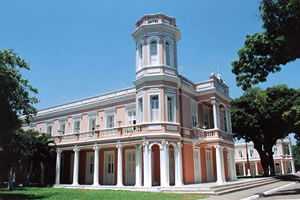
\includegraphics[width=16cm]{figuras/exemplo-1}
%		}{
%			\Fonte{\citeonline[p.~5]{UFC2012}.}
%		}	
%	\end{figure}
	
 %   Texto1 texto texto texto texto texto texto texto texto texto texto texto texto texto texto texto texto texto texto texto texto texto texto texto texto texto texto texto texto texto texto texto texto texto texto texto texto texto texto texto texto texto texto texto texto1.

%    Texto2 texto texto texto texto texto texto texto texto texto texto texto texto texto texto texto texto texto texto. Texto texto texto texto texto texto texto texto texto texto texto texto texto texto texto texto texto texto texto2.

 %   Texto3 texto texto texto texto texto texto texto texto texto texto texto texto texto texto texto texto texto texto. Texto texto texto texto texto texto texto texto texto texto texto texto texto texto texto texto texto texto texto3.

  %  Texto4 texto texto texto texto texto texto texto texto texto texto texto texto texto texto texto texto texto texto. Texto texto texto texto texto texto texto texto texto texto texto texto texto texto texto texto texto texto texto4.

 %   A Figura \ref{fig:sondas} texto texto texto texto texto texto texto texto texto texto texto texto texto texto texto texto texto texto texto. Texto texto texto texto texto texto texto texto texto texto texto texto texto texto texto texto texto texto texto3.

%	\begin{figure}[h!]
%		\centering
%		\captionsetup{width=14cm}%Da mesma largura que a figura
%		\Caption{\label{fig:sondas} Gráfico da atmosfera superior}	
%		\UFCfig{}{
%			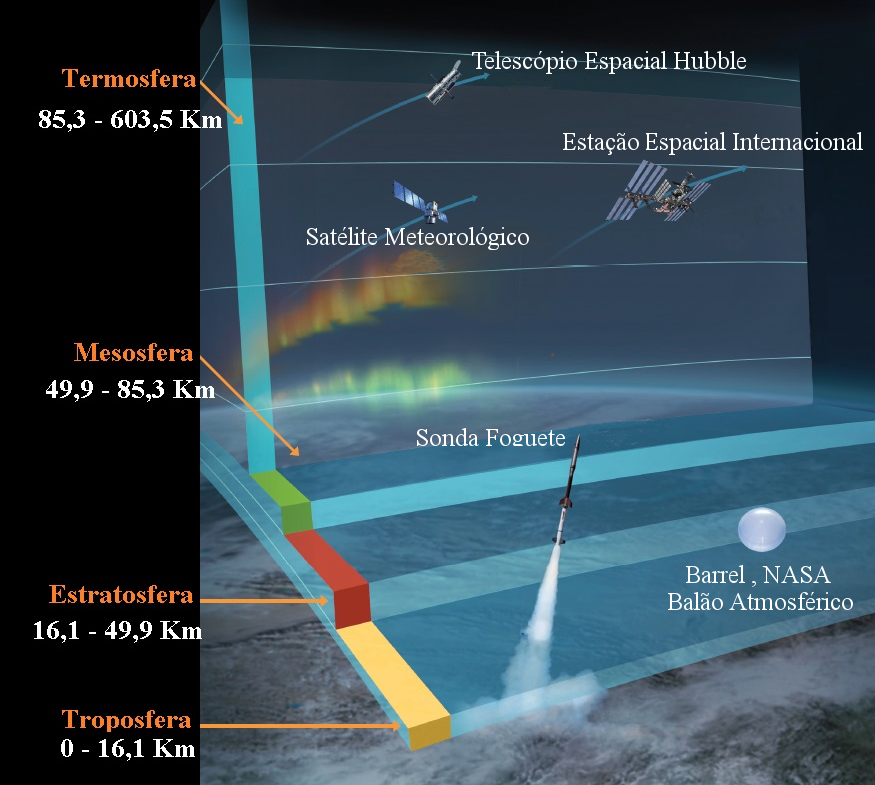
\includegraphics[width=14cm]{figuras/sondas}
%		}{
%			\Fonte{adaptado da \citeonline[p.~98]{NASA2016}.}}	
%	\end{figure}
%
 %   Texto5 texto texto texto texto texto texto texto texto texto texto texto texto texto texto texto texto texto texto texto texto texto texto texto texto texto texto texto texto texto texto texto texto texto texto texto texto texto texto texto texto texto texto texto texto5.

 %   Texto6 texto texto texto texto texto texto texto texto texto texto texto texto texto texto texto texto texto texto texto texto texto texto texto texto texto texto texto texto texto texto texto texto texto texto texto texto texto texto texto texto texto texto texto texto5.

 %   Texto7 texto texto texto texto texto texto texto texto texto texto texto texto texto texto texto texto texto texto texto texto texto texto texto texto texto texto texto texto texto texto texto texto texto texto texto texto texto texto texto texto texto texto texto texto texto texto texto texto texto texto texto texto texto texto texto texto texto texto texto texto texto texto texto6.

 %   Evite terminar seções, capítulos e etc com figura. Procure escrever mais.

%\section{Inserindo tabelas}\label{sec:tabelas}
    
%    A Tabela \ref{tab:exemplo-1}... texto texto texto texto texto texto texto texto texto texto texto texto texto texto texto texto texto texto texto. Texto texto texto texto texto texto texto texto texto texto texto texto texto texto texto texto texto texto texto.
	


	%\begin{table}[h!]	
	%	\centering
	%	\Caption{\label{tab:exemplo-1} Exemplo de tabela}	
	%	\UFCtab{}{
	%		\begin{tabular}{cll}
	%			\toprule
	%			Ranking & Exon Coverage & Splice Site Support \\
	%			\midrule \midrule
	%			E1 & Complete coverage by a single transcript & Both splice sites\\
	%			E2 & Complete coverage by more than a single transcript & Both splice sites\\
	%			E3 & Partial coverage & Both splice sites\\
	%			E4 & Partial coverage & One splice site\\
	%			E5 & Complete or partial coverage & No splice sites\\
	%			E6 & No coverage & No splice sites\\
	%			\bottomrule
	%		\end{tabular}
	%	}{
	%	\Fonte{elaborado pelo autor.}
	%}
	%\end{table}




  
%\subsection{Uso de siglas} \label{sec:siglas}

%    Para utilizar siglas, primeiro defina a sigla no arquivo "lista-de-abreviaturas-e-siglas"~ dentro da pasta "1-pre-textuais" com o comando 
%    \begin{verbatim}
 %       \newacronym{ABNT}{ABNT}{Associação Brasileira de Normas Técnicas}
 %   \end{verbatim}
%    Depois chame a sigla com o comando:
 %   \begin{verbatim}
%        \gls{ABNT}
%    \end{verbatim}
 %   Fica assim: \gls{ABNT}. A primeira vez que o comando é usado para uma determinada sigla, aparece o significado por extenso da sigla com a sua abreviação em seguida. A partir da segunda vez que o comando para uma determinada sigla é usado, aparace apenas a sigla. Por exemplo: \gls{ABNT}.  
    
 %   Veja o código fonte de outros exemplos: Teste de siglas \gls{TEST}, outros exemplos de siglas: \gls{DA}, \gls{MCEG}. 
  %  Repare que sempre as siglas estão sendo definidas primeiramente no arquivo ``lista-de-abreviaturas-e-siglas''.
    
%\subsubsection{Exemplo de subseção quaternária} \label{sec:quater}

%Texto texto texto texto texto texto texto texto texto texto texto texto texto texto texto texto texto texto texto texto texto texto texto texto texto texto texto texto texto texto texto texto texto texto texto texto texto texto texto texto texto texto texto texto texto.

%\subsubsubsection{Exemplo de subseção quinária} 

%Texto texto texto texto texto texto texto texto texto texto texto texto texto texto texto texto texto texto texto texto texto texto texto texto texto texto texto texto texto texto texto texto texto texto texto texto texto texto texto texto texto texto texto texto texto.

\nocite{ibge,introducao-ta, pcd-mercado-trabalho, abnt, laramara, secretaria, dorina, cadevi}
